\documentclass{iopconfser}

\usepackage{amsmath,amssymb}
\usepackage{graphicx}
\usepackage{booktabs}
\usepackage{siunitx}
\usepackage{subcaption}
\usepackage{tikz}
\usepackage{pgfplots}
\usepackage{algorithm}
\usepackage{algpseudocode}
\usepackage{placeins}
\usepackage{hyperref}

\usetikzlibrary{arrows.meta, positioning, shapes.geometric, calc}
\usepgfplotslibrary{groupplots}
\pgfplotsset{compat=1.18}

\setcounter{topnumber}{5}
\setcounter{bottomnumber}{5}
\setcounter{totalnumber}{8}
\renewcommand{\topfraction}{0.9}
\renewcommand{\bottomfraction}{0.8}
\renewcommand{\textfraction}{0.07}
\renewcommand{\floatpagefraction}{0.85}

\hypersetup{colorlinks=true,linkcolor=blue,citecolor=blue,urlcolor=blue}

\sisetup{
  detect-all,
  per-mode=symbol
}

\begin{document}

\title{Sensitivity of Flame Transfer Functions to Geometry Changes in a Laminar Premixed Slot Burner}
% \author{Alessandro Giannotta$^{1}$, Stefania Cherubini$^{1}$, Pietro De Palma$^{1}$}
\author{}
% \affil{$^{1}$Department of Mechanics, Mathematics and Management, Politecnico di Bari, Bari, Italy}
% \email{alessandro.giannotta@poliba.it}

\begin{abstract}
Flame transfer functions provide a compact description of the coupling between inlet-flow perturbations and unsteady heat release, but their numerical reconstruction over broad frequency ranges and across geometry variations remains computationally expensive. This work presents a SU2-based workflow for reconstructing the flame transfer function of a laminar premixed slot-burner flame using a flamelet-generated-manifold combustion model, broadband chirp forcing, and frequency-domain processing of the global heat-release signal. The baseline configuration follows the slot-burner flame of Contini et al., while free-form deformation is used to introduce controlled convergent and divergent modifications of the burner lip. A single chirp-forced transient simulation recovers the baseline gain and phase over the frequency range of interest. The baseline response exhibits near-unity low-frequency gain, a moderate mid-frequency amplification, and high-frequency roll-off associated with convective filtering. Lip deformation modifies both the amplitude and timing of the response. The convergent geometry increases the main gain peak and shifts it to higher frequency, whereas the divergent geometry suppresses the peak and reduces the phase lag over part of the band. These trends show that small changes in the anchoring region can significantly modify the effective convective delay and the spatial coherence of heat-release fluctuations. The workflow provides a direct-simulation foundation for future adjoint-based geometry optimization of thermoacoustic response.
\end{abstract}

\section{Introduction}
\label{sec:introduction}

Thermoacoustic instabilities remain a central challenge in low-emission combustion systems because constructive coupling between unsteady heat release and the acoustic field can drive large pressure oscillations \cite{lieuwen2012unsteady,poinsot2005theoretical,poinsot2017prediction}. Their onset is strongly sensitive to flame dynamics, geometry, and operating conditions, so small changes in the flame response can move a combustor toward or away from instability \cite{mongia2003challenges}. This sensitivity is evident in both canonical and application-oriented thermoacoustic configurations, including systems previously studied by the present authors \cite{Giannotta2022,abbot2021thermoacoustic}. A compact way to characterize the flame side of this feedback loop is the Flame Transfer Function (FTF), which relates inlet-flow perturbations to the fluctuating heat-release response over a frequency range of interest.

Reliable FTF prediction remains difficult. Experimental observables often provide indirect information on the heat-release dynamics, and optical diagnostics require additional processing to obtain a consistent global transfer function \cite{han2015spatial,yuan2015reaction}. On the numerical side, repeated single-frequency forcing calculations provide clean transfer-function estimates, but broad spectral coverage requires many transient simulations. Broadband forcing, and in particular chirp excitation, offers a more efficient route by exciting a wide range of frequencies in a single calculation, after which the flame response can be reconstructed in the frequency domain \cite{schuller2002modelling}.

Predictive thermoacoustic design also requires models with physical content and reliable sensitivity information. Adjoint methods are especially powerful in this context because they make sensitivity analysis, gradient evaluation, and parameter inference tractable even when the model space is high-dimensional \cite{albring2016efficient,magri2013sensitivity,aguilar2017adjoint,aguilar2020thermoacoustic}. Bayesian inference provides a complementary route for calibrating physics-based thermoacoustic models against data while quantifying uncertainty \cite{juniper2022JSV,Yoko2023}. In recent work, Giannotta et al. showed how flame-response modeling benefits from physically interpretable kinematic mechanisms \cite{GiannottaCnF2023} and how adjoint-accelerated Bayesian inference can obtain quantitatively accurate flame models from forced-response data \cite{giannotta2025bayesian}. These developments motivate a design chain in which calibrated models and adjoint gradients are used to tailor the FTF and weaken flame-acoustic feedback.

The present work addresses the CFD component of that broader program. We use SU2 as the simulation platform and a Flamelet Generated Manifold (FGM) combustion closure to model a laminar premixed slot-burner flame following the configuration studied by Contini et al. \cite{palacios2013su2,vanOijen2000fgm,contini2020slotburner}. Geometry variation is introduced through Free Form Deformation (FFD), which provides a smooth and compact parametrization of burner-shape changes \cite{sederberg1986ffd}. The workflow combines FGM-based reacting-flow simulation, broadband chirp forcing, frequency-domain reconstruction of the FTF from the global heat-release-rate signal, and systematic comparison across deformed geometries. Its implementation within SU2 keeps the direct simulations, geometry parameterization, and signal-processing chain aligned with the code's discrete-adjoint infrastructure and CoDiPack-based automatic-differentiation machinery.

The contribution of this paper is a reproducible direct-simulation workflow that reconstructs a broadband FTF and uses it to quantify the effect of localized burner-lip deformations on gain and phase. The paper identifies how convergent and divergent modifications redistribute the response in frequency and clarifies why the near-anchoring region is an effective target for future geometry optimization.

The remainder of the paper is organized as follows. Section~\ref{sec:methodology} describes the numerical methodology. Section~\ref{sec:results} presents the baseline flame and the geometry-dependent FTF trends. Section~\ref{sec:conclusions} summarizes the findings and outlines future directions.

\section{Numerical Methodology}
\label{sec:methodology}

\subsection{Governing Equations and FGM Model}
\label{subsec:fgm}

The flow is modeled using the compressible reacting Navier--Stokes equations together with a flamelet-generated manifold closure. In conservative form, the governing system is written as
\begin{equation}
  \frac{\partial \mathbf{U}}{\partial t}
  + \nabla \cdot \mathbf{F}_{\mathrm{inv}}(\mathbf{U})
  - \nabla \cdot \mathbf{F}_{\mathrm{vis}}(\mathbf{U},\nabla \mathbf{U})
  = \mathbf{S}(\mathbf{U},\boldsymbol{\psi}),
  \label{eq:governing-equations}
\end{equation}
where $\mathbf{U}$ denotes the transported conservative variables, $\mathbf{F}_{\mathrm{inv}}$ and $\mathbf{F}_{\mathrm{vis}}$ denote the inviscid and viscous fluxes, and $\mathbf{S}$ contains the combustion source terms and closure contributions associated with the manifold variables.

\begin{align}
  \frac{\partial \rho}{\partial t} + \nabla \cdot (\rho \mathbf{u}) &= 0, \label{eq:continuity}\\
  \frac{\partial (\rho \mathbf{u})}{\partial t} + \nabla \cdot (\rho \mathbf{u}\otimes\mathbf{u} + p\mathbf{I} - \boldsymbol{\tau}) &= 0, \label{eq:momentum}\\
  \frac{\partial (\rho h_t)}{\partial t} + \nabla \cdot \bigl(\mathbf{u}(\rho h_t + p)\bigr) &= \nabla \cdot (k \nabla T) + \dot{\omega}_T, \label{eq:energy}
\end{align}
where $\rho$ is the density, $\mathbf{u}$ is the velocity vector, $p$ is pressure, $\boldsymbol{\tau}$ is the viscous stress tensor, $h_t$ is total enthalpy, $k$ is the thermal conductivity, $T$ is temperature, and $\dot{\omega}_T$ denotes the volumetric heat-release contribution.

In an FGM framework, transported scalar variables parameterize the thermochemical state through table lookup. For the present Contini configuration, the manifold is defined in terms of progress variable and total enthalpy, with the progress-variable source term and global heat release also tabulated. The progress variable is based on the species mass fractions of H$_2$, H$_2$O, CO, and CO$_2$, and the tabulated ranges cover approximately $[0,\,2.753279\times10^{-1}]$ for the progress variable and $[-3.081484\times10^{6},\,-1.565767\times10^{5}]$ for total enthalpy.

A generic representation is
\begin{equation}
  \boldsymbol{\psi} = \left(\psi_1,\psi_2,\dots,\psi_m\right),
  \qquad
  \mathbf{q} = \mathcal{M}\!\left(\boldsymbol{\psi}\right),
  \label{eq:fgm-lookup}
\end{equation}
where $\boldsymbol{\psi}$ contains the manifold coordinates, $\mathbf{q}$ denotes the thermochemical state, and $\mathcal{M}$ is the precomputed flamelet table.
The table provides temperature, species mass fractions, transport properties, and source terms as functions of the manifold coordinates \cite{vanOijen2000fgm}.

Figure~\ref{fig:lut-occupancy} illustrates the manifold used in the present simulations together with the distribution of sampled solution states. The occupied region confirms that the flame mainly evolves over a restricted portion of the tabulated space, while the spread toward lower enthalpy is associated with cells close to the burner walls, where heat losses drive the thermochemical state away from the adiabatic branch.

\begin{figure}[!htbp]
  \centering
  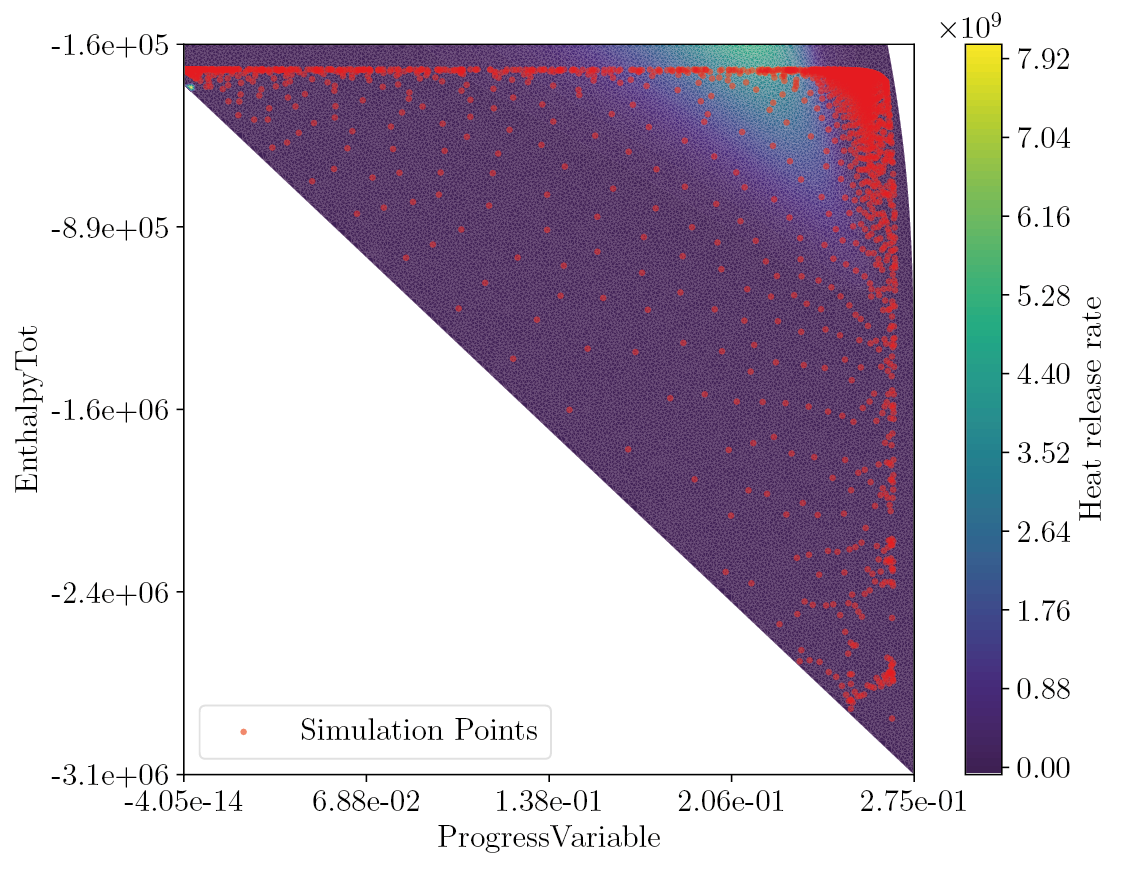
\includegraphics[width=0.82\linewidth]{LUT.png}
  \caption{FGM lookup table in progress-variable/enthalpy space overlaid with the states sampled by the transient solution. Most states remain on a restricted portion of the manifold, while the low-enthalpy branch is populated by cells close to the cooled walls, where heat losses move the local thermochemical state away from the adiabatic trajectory.}
  \label{fig:lut-occupancy}
\end{figure}
\FloatBarrier

\subsection{Slot-Burner Flame Configuration}
\label{subsec:bunsen}

The considered configuration is a two-dimensional laminar premixed slot-burner flame using a methane/air mixture at equivalence ratio $\phi=1$ and burner temperature $298\,\mathrm{K}$. The setup follows the slot-burner configuration reported by Contini et al. \cite{contini2020slotburner}. The case is characterized by a mean inlet velocity of $0.7\,\mathrm{m\,s^{-1}}$ and an initial velocity field of $(0.7,0,0)\,\mathrm{m\,s^{-1}}$. This operating point isolates the effect of inlet forcing and geometry deformation on the global flame response.

\begin{table}[!htbp]
  \centering
  \caption{Baseline slot-burner flame configuration.}
  \label{tab:baseline-conditions}
  \begin{tabular}{@{}p{0.43\linewidth}p{0.47\linewidth}@{}}
    \toprule
    Quantity & Value \\
    \midrule
    Fuel/oxidizer mixture & Methane/air \\
    Equivalence ratio, $\phi$ & 1 \\
    Inlet temperature & $298\,\mathrm{K}$ \\
    Ambient pressure & Zero gauge pressure at the outlet \\
    Mean inlet velocity, $\bar{u}$ & $0.7\,\mathrm{m\,s^{-1}}$ \\
    Characteristic mesh size & Two-dimensional unstructured mesh used for the verification case \\
    Domain dimensions & Burner geometry and near-field domain used for the verification case \\
    Boundary-condition type & Isothermal wall, symmetry, inlet profile, pressure outlet \\
    \bottomrule
  \end{tabular}
\end{table}

The direct case uses a specified inlet profile. The remaining boundary conditions are an isothermal wall at $298\,\mathrm{K}$, a symmetry boundary on the lateral side, and a pressure outlet with zero gauge pressure. The scalar transport is initialized and clipped using the flamelet quantities listed above, and the direct run monitors global heat release in the history output.

The implementation is kept inside the SU2 framework so that the same infrastructure can support future discrete-adjoint evaluations. Automatic differentiation through CoDiPack provides the basis for propagating geometry and model sensitivities consistently once the optimization loop is activated.

\begin{figure}[!htbp]
  \centering
  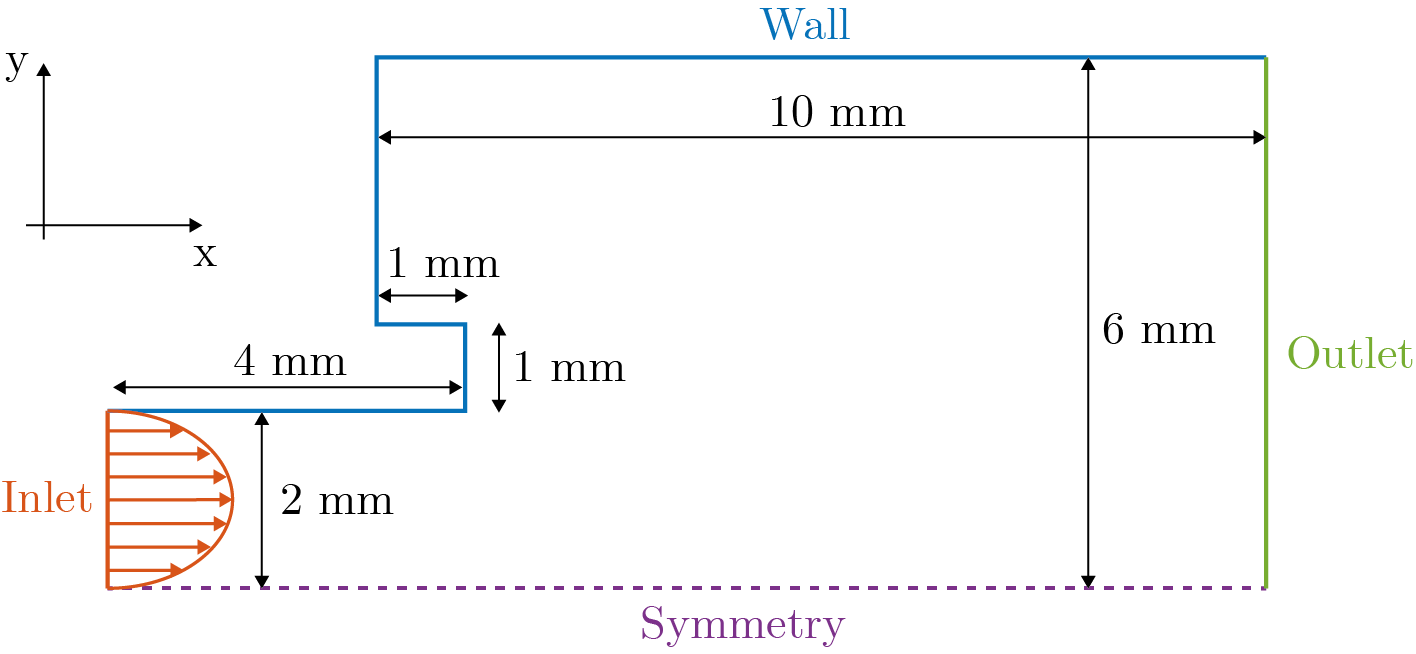
\includegraphics[width=0.74\linewidth]{GeometricSetup.png}
  \caption{Baseline slot-burner configuration adopted in the present study. The geometry reproduces the reference layout of the Contini configuration and defines the lip region that is later modified through FFD.}
  \label{fig:baseline-geometry}
\end{figure}
\FloatBarrier

\subsection{Geometry Parameterization Using FFD}
\label{subsec:ffd}

Geometry variations are generated with Free Form Deformation, which embeds the burner surface in a structured control lattice and deforms the shape by displacing selected control points \cite{sederberg1986ffd}. This approach preserves smoothness and provides a compact parametrization for systematic studies. In the present case the FFD box is defined by the 2D corner coordinates $(-2\,\mathrm{mm},\,1.8\,\mathrm{mm})$, $(1\,\mathrm{mm},\,1.8\,\mathrm{mm})$, $(1\,\mathrm{mm},\,3.5\,\mathrm{mm})$, and $(-2\,\mathrm{mm},\,3.5\,\mathrm{mm})$, with FFD degree $(2,1,0)$. The representative deformations examined below correspond to prescribed in-plane control-point displacements that produce either a convergent or a divergent lip shape.

Let $\mathbf{P}_{ijk}$ denote the control points of the FFD lattice. A deformed point $\mathbf{x}'$ can be written generically as
\begin{equation}
  \mathbf{x}' = \sum_{i=0}^{l}\sum_{j=0}^{m}\sum_{k=0}^{n} B_i^{l}(\xi)\,B_j^{m}(\eta)\,B_k^{n}(\zeta)\,\mathbf{P}_{ijk},
  \label{eq:ffd-mapping}
\end{equation}
where $B_i^l$ are Bernstein polynomials and $(\xi,\eta,\zeta)$ are the local coordinates inside the FFD box.

The zero-displacement configuration recovers the baseline geometry, while the prescribed control-point displacements define the deformed cases. Figure~\ref{fig:ffd-geometries} compares the undeformed burner with a representative FFD-modified shape.

\begin{figure}[!htbp]
  \centering
  \begin{subfigure}[t]{0.48\linewidth}
    \centering
    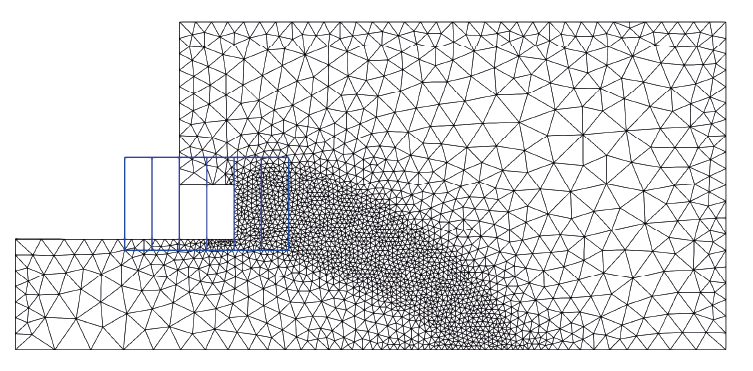
\includegraphics[width=\linewidth]{baseline_geometry.png}
    \caption{Baseline geometry.}
    \label{fig:ffd-baseline}
  \end{subfigure}
  \hfill
  \begin{subfigure}[t]{0.48\linewidth}
    \centering
    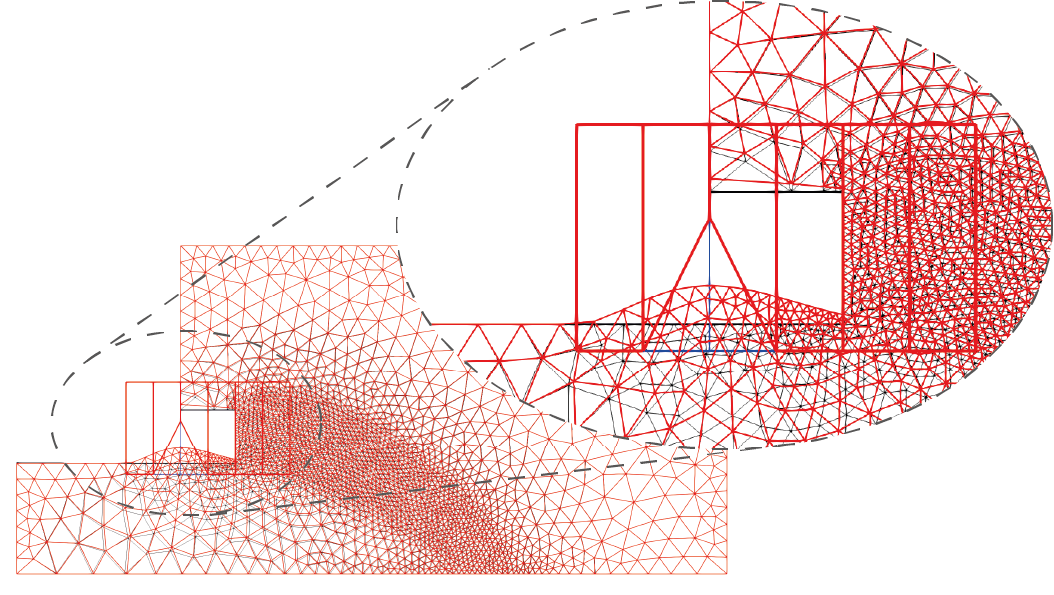
\includegraphics[width=\linewidth]{deformed_geometry.png}
    \caption{Example deformed geometry.}
    \label{fig:ffd-deformed}
  \end{subfigure}
  \caption{Baseline and representative FFD-deformed burner geometries. The imposed control-point displacements modify the burner lip smoothly while preserving a common geometric parametrization across cases.}
  \label{fig:ffd-geometries}
\end{figure}
\FloatBarrier

\subsection{Broadband Chirp Excitation}
\label{subsec:chirp}

To reduce the number of single-frequency runs, the inlet velocity is perturbed using a broadband chirp signal. The chirp amplitude is $A=0.01$, the sweep spans from $2\,\mathrm{Hz}$ to $180\,\mathrm{Hz}$, the duration is $1.5\,\mathrm{s}$, the start time is $0\,\mathrm{s}$, the initial phase is $\pi/2$, and the chirp is linear in frequency. A generic form is
\begin{equation}
  u_{\mathrm{in}}(t) = \bar{u}\left[1 + A \sin\bigl(\phi(t)\bigr)\right],
  \label{eq:inlet-chirp}
\end{equation}
where $\bar{u}$ is the mean inlet velocity, $A$ is the nondimensional perturbation amplitude, and $\phi(t)$ is the chirp phase. The instantaneous frequency is obtained from
\begin{equation}
  f(t) = \frac{1}{2\pi}\frac{\mathrm{d}\phi}{\mathrm{d}t}.
  \label{eq:instantaneous-frequency}
\end{equation}

The forcing amplitude is kept small so that the reconstructed response is representative of the linear transfer function over the frequency band of interest. For the time-series analysis reported here, the first second of the record is discarded to remove the start-up transient, and the inlet velocity together with the global heat-release rate are normalized by their mean values over the retained window. Figure~\ref{fig:chirp-signal} reports the resulting baseline input-output signals.

\begin{figure}[!htbp]
  \centering
  \begin{tikzpicture}
    \begin{groupplot}[
      group style={group size=1 by 2, vertical sep=3.2em},
      width=0.88\linewidth,
      height=0.22\linewidth,
      xmin=0,
      xmax=1.351,
      grid=both,
      major grid style={gray!15},
      minor grid style={gray!08},
      tick align=outside,
      tick pos=left,
      enlargelimits=false,
      axis line style={black, very thick},
      label style={font=\small},
      tick label style={font=\small},
      title style={font=\small}
    ]
      \nextgroupplot[
        ylabel={$u_{\mathrm{in}}/\overline{u}_{\mathrm{in}}$},
        ymin=0.99,
        ymax=1.01,
        xticklabels=\empty
      ]
      \addplot[blue!75!black, very thick] table[col sep=comma, x=time_s, y=u_norm] {signal_baseline.csv};

      \nextgroupplot[
        xlabel={Time [s]},
        ylabel={$Q/\overline{Q}$},
        ymin=0.99,
        ymax=1.01
      ]
      \addplot[red!75!black, very thick] table[col sep=comma, x=time_s, y=qdot_norm] {signal_baseline.csv};
    \end{groupplot}
  \end{tikzpicture}
  \caption{Baseline chirp input and corresponding global heat-release-rate response, both normalized by their mean values after removal of the initial transient. The bounded fluctuations confirm that the forcing remains in a weakly perturbed regime suitable for linear transfer-function reconstruction.}
  \label{fig:chirp-signal}
\end{figure}
\FloatBarrier

\subsection{Global Heat-Release-Rate Extraction}
\label{subsec:heat-release}

The flame response is quantified through the global heat-release rate,
\begin{equation}
  Q(t) = \int_{\Omega} \dot{\omega}_T(\mathbf{x},t)\,\mathrm{d}\Omega,
  \label{eq:global-heat-release}
\end{equation}
where $\Omega$ denotes the flame domain and $\dot{\omega}_T$ is the local volumetric heat-release rate. The fluctuating component is obtained as
\begin{equation}
  Q'(t) = Q(t) - \overline{Q},
  \qquad
  u'(t) = u_{\mathrm{in}}(t) - \overline{u}_{\mathrm{in}},
  \label{eq:fluctuations}
\end{equation}
with overbars indicating suitable time averages or reference values over the analysis window.

The heat-release signal is sampled consistently with the time step used in the transient solver. Mean removal, transient rejection, and spectral processing are applied over the same analysis window for all geometries so that the reported differences can be attributed to changes in flame response.

\subsection{FTF Reconstruction}
\label{subsec:ftf}

The FTF is reconstructed from the frequency-domain ratio of the fluctuating heat-release and inlet-velocity signals:
\begin{equation}
  F(f) = \frac{\hat{Q}'(f)}{\hat{u}'(f)},
  \label{eq:ftf-definition}
\end{equation}
where the hat denotes the Fourier transform. The gain is given by $|F(f)|$ and the phase by $\arg(F(f))$.

The post-processing uses the same reconstruction procedure for the baseline and deformed cases. The analysis window begins after an initial transient and spans the last 1.351 seconds of the 1.5 second simulation, which provides the frequency-domain input-output data used to compare gain and phase across geometries.

\begin{algorithm}[!htbp]
  \caption{Broadband FTF reconstruction workflow.}
  \label{alg:workflow}
  \begin{algorithmic}[1]
    \State Initialize baseline or FFD-deformed geometry.
    \State Run a steady or transient preconditioning simulation until the flame is established.
    \State Apply the chirp forcing at the inlet.
    \State Record $u_{\mathrm{in}}(t)$ and $Q(t)$ over the analysis window.
    \State Remove means and optional trends to obtain $u'(t)$ and $Q'(t)$.
    \State Compute FFTs, $\hat{u}'(f)$ and $\hat{Q}'(f)$.
    \State Evaluate $F(f)=\hat{Q}'(f)/\hat{u}'(f)$.
    \State Extract gain $|F(f)|$ and phase $\arg(F(f))$ for reporting.
  \end{algorithmic}
\end{algorithm}
\FloatBarrier

\section{Results and Discussion}
\label{sec:results}

The results first establish the baseline flame behavior and then assess how selected FFD-induced deformations modify the reconstructed flame transfer function. The discussion focuses on relative changes in gain, phase, and peak frequency because these quantities determine whether a flame response is likely to reinforce or weaken an acoustic feedback loop.

\subsection{Baseline Steady Flame}
\label{subsec:baseline-steady}

The baseline configuration is characterized first in terms of the steady temperature and heat-release-rate distributions. These fields identify the stabilization region, the overall flame extent, and the near-lip flame structure that determines the subsequent dynamic response. The heat-release field is concentrated in a thin layer anchored at the burner lip, so perturbations imposed at the inlet influence the global heat release primarily through their effect on the flame root and on the subsequent convection of disturbances along the flame front. Consistently with the manifold occupancy shown in Figure~\ref{fig:lut-occupancy}, the near-wall regions occupy lower-enthalpy states because heat losses at the cooled boundaries locally weaken the flame and pull the solution away from the adiabatic branch.

\begin{figure}[!htbp]
  \centering
  \begin{subfigure}[t]{0.48\linewidth}
    \centering
    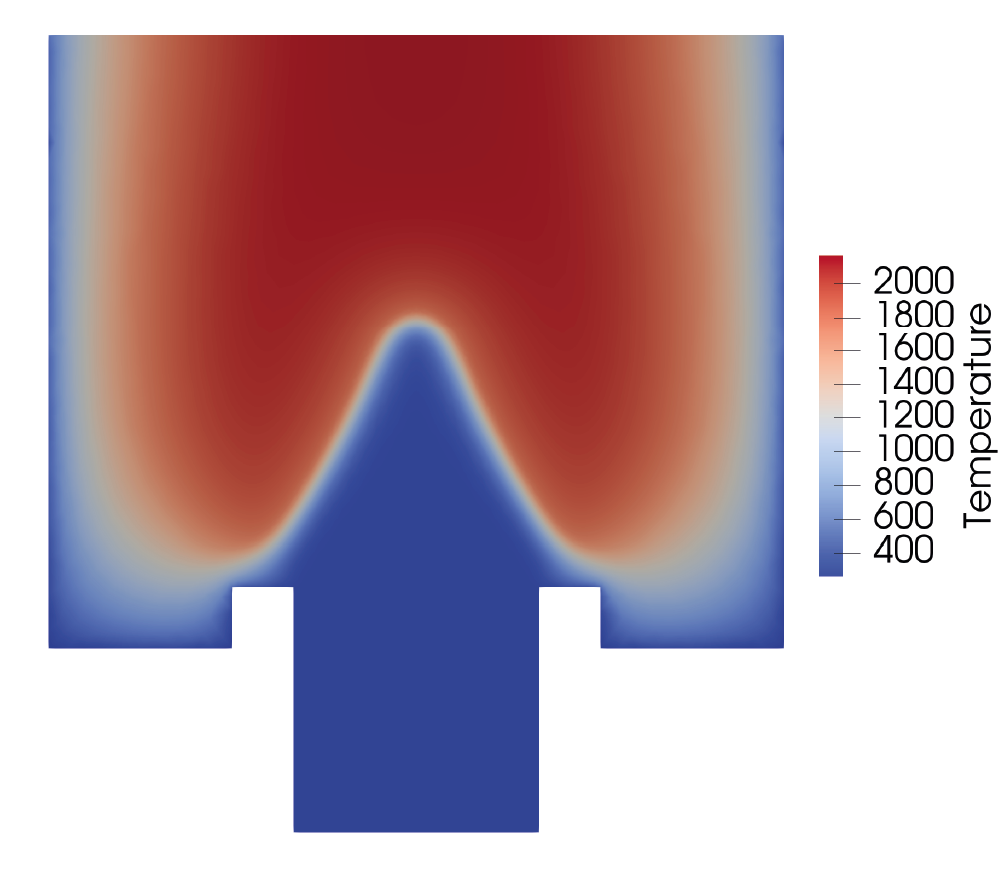
\includegraphics[width=\linewidth]{Temperature.png}
    \caption{Temperature field.}
    \label{fig:steady-temperature}
  \end{subfigure}
  \hfill
  \begin{subfigure}[t]{0.48\linewidth}
    \centering
    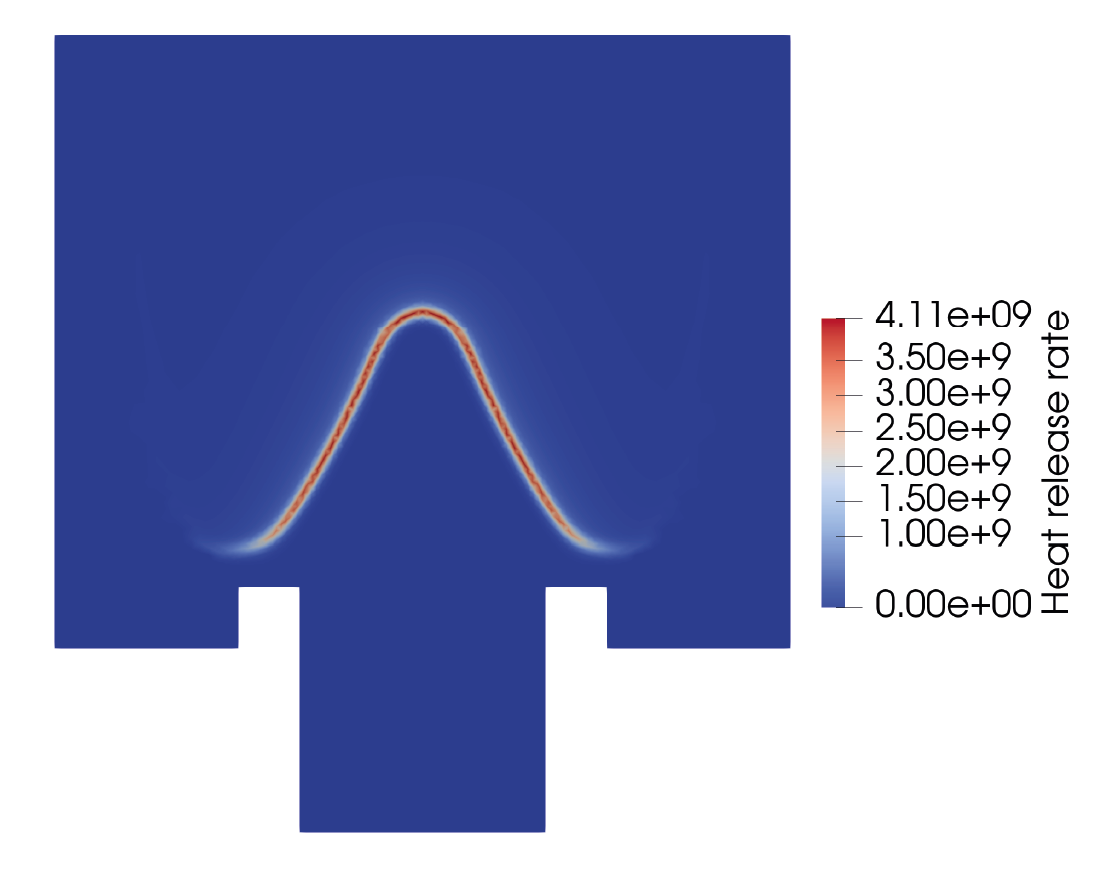
\includegraphics[width=\linewidth]{HeatReleaseRate.png}
    \caption{Heat-release-rate field.}
    \label{fig:steady-hrr}
  \end{subfigure}
  \caption{Baseline steady-flame structure. The temperature field shows the global flame envelope, whereas the heat-release-rate field identifies the thinner reactive layer anchored at the burner lip and extending downstream along the shear layer.}
  \label{fig:steady-flame}
\end{figure}
\FloatBarrier

\subsection{Baseline Chirp Response}
\label{subsec:baseline-chirp}

The transient response to broadband inlet forcing is shown in Figure~\ref{fig:chirp-signal}. Once the initial transient is removed, both the normalized inlet velocity and the normalized heat-release signal remain within approximately $\pm 1\%$ of their mean values. The heat-release response follows the imposed chirp without large amplitude excursions, which indicates that the calculation probes the small-signal dynamics of the anchored flame. This regime is appropriate for reconstructing a linear FTF because the measured gain and phase reflect the flame's response to the input perturbation around a nearly unchanged mean operating state.

\subsection{Baseline FTF}
\label{subsec:baseline-ftf}

Figure~\ref{fig:baseline-ftf} reports the reconstructed baseline transfer function in terms of gain and phase. The response is close to unity at the lowest frequencies, reaches a moderate peak of about $1.04$ near $46\,\mathrm{Hz}$, and then decays progressively toward higher frequencies. This shape is characteristic of a convectively dominated premixed flame response. Slow inlet perturbations are transmitted efficiently because the flame can adjust quasi-steadily, while high-frequency disturbances are attenuated as their wavelength becomes short relative to the convective distance between the inlet, the stabilization region, and the distributed heat-release zone. The phase becomes progressively more negative with frequency, which is consistent with an effective transport delay between the inlet perturbation and the integrated heat-release response.

\begin{figure}[!htbp]
  \centering
  \begin{tikzpicture}
    \begin{groupplot}[
      group style={group size=1 by 2, vertical sep=1.8em},
      width=0.88\linewidth,
      height=0.23\linewidth,
      xmin=0,
      xmax=140,
      grid=both,
      major grid style={gray!15},
      minor grid style={gray!08},
      tick align=outside,
      tick pos=left,
      enlargelimits=false,
      axis line style={black, thick},
      label style={font=\small},
      tick label style={font=\small}
    ]
      \nextgroupplot[
        ylabel={Gain $|F(f)|$},
        ymin = 0.3,
        ymax=1.08,
        xticklabels=\empty
      ]
      \addplot[blue!75!black, thick] table[col sep=comma, x=frequency_Hz, y=FTF_amp] {FTF_baseline.csv};

      \nextgroupplot[
        xlabel={Frequency [Hz]},
        ymin=-1.4,
        ymax=0.05,
        ylabel={Phase [rad]}
      ]
      \addplot[blue!75!black, thick] table[col sep=comma, x=frequency_Hz, y=FTF_phase_rad] {FTF_baseline.csv};
    \end{groupplot}
  \end{tikzpicture}
  \caption{Baseline flame transfer function reconstructed from the chirp-forced direct simulation. The gain exhibits a clear mid-band maximum before rolling off at higher frequency, while the phase shows the progressive lag associated with transport and flame-response delays.}
  \label{fig:baseline-ftf}
\end{figure}
\FloatBarrier

\subsection{Effect of FFD Geometry Variations}
\label{subsec:geometry-variations}

To illustrate the sensitivity of the flame response to burner-shape modifications, the baseline configuration is compared with two representative FFD-deformed cases. The selected deformations act on the lip region, where the flame anchors and where velocity perturbations first interact with the reacting layer. This region is dynamically important because changes in local passage area modify the mean acceleration, the convective time scale, and the way inlet perturbations wrinkle or displace the flame root. The two cases therefore provide a controlled test of how localized geometric changes redistribute the FTF in frequency.

Table~\ref{tab:geometry-cases} summarizes the considered geometries and their main characteristics.

\begin{table}[!htbp]
  \centering
  \caption{Representative geometry cases generated through FFD.}
  \label{tab:geometry-cases}
  \small
  \setlength{\tabcolsep}{4pt}
  \renewcommand{\arraystretch}{1.15}
  \begin{tabular}{@{}p{0.12\linewidth}p{0.27\linewidth}p{0.29\linewidth}p{0.20\linewidth}@{}}
    \toprule
    Case & FFD setting & Geometry change & Passage effect \\
    \midrule
    Baseline & Zero displacement & Reference lip geometry & Nominal passage \\
    Case 1 & Convergent shift, $\pm 0.5\,\mathrm{mm}$ & Inward lip deformation & Local contraction near the flame root \\
    Case 2 & Divergent shift, $\pm 0.5\,\mathrm{mm}$ & Outward lip deformation & Local expansion near the flame root \\
    \bottomrule
  \end{tabular}
\end{table}

Figures~\ref{fig:geometry-comparison} and \ref{fig:geometry-ftf-comparison} compare the selected deformed configurations and their transfer functions against the baseline flame. The relevant design information is contained in the relative changes: shifts in gain level, modification of phase lag, and redistribution of spectral features that may be favorable from a thermoacoustic-design perspective.

\begin{figure}[!htbp]
  \centering
  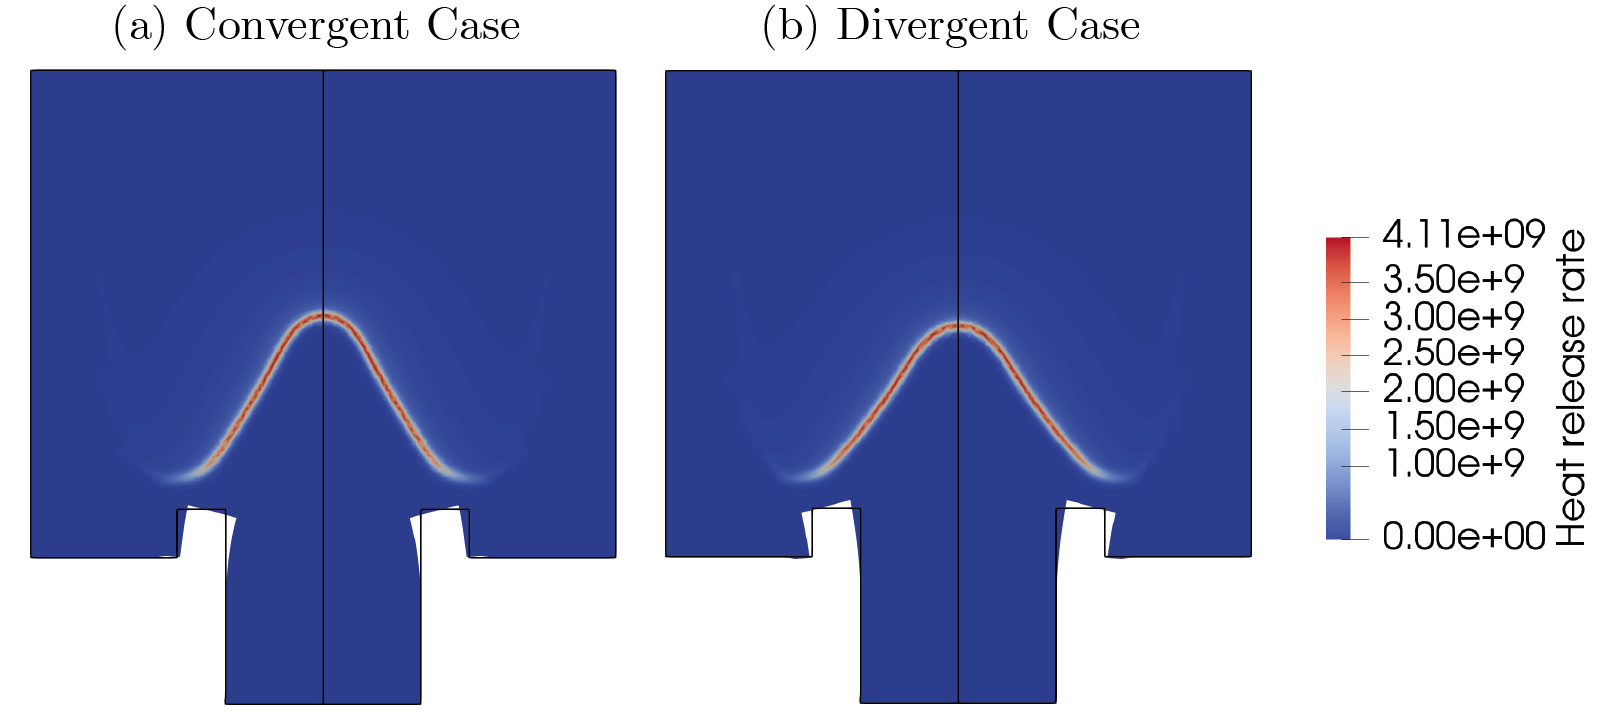
\includegraphics[width=0.92\linewidth]{Deformed_Cases.png}
  \caption{Representative FFD-deformed burner geometries used in the comparison. The convergent case contracts the near-root passage, whereas the divergent case opens it, thereby modifying the flow field seen by the anchored flame.}
  \label{fig:geometry-comparison}
\end{figure}

\begin{figure}[!htbp]
  \centering
  \begin{tikzpicture}
    \begin{groupplot}[
      group style={group size=1 by 2, vertical sep=1.8em},
      width=0.88\linewidth,
      height=0.23\linewidth,
      xmin=0,
      xmax=140,
      grid=both,
      major grid style={gray!15},
      minor grid style={gray!08},
      tick align=outside,
      tick pos=left,
      enlargelimits=false,
      axis line style={black, thick},
      label style={font=\small},
      tick label style={font=\small},
      legend style={
        font=\small,
        draw=none,
        at={(0.5,1.22)},
        anchor=south,
        legend columns=3
      }
    ]
      \nextgroupplot[
        ylabel={Gain $|F(f)|$},
        ymin=0.0,
        ymax=1.1,
        xticklabels=\empty
      ]
      \addplot[blue!75!black, thick] table[col sep=comma, x=frequency_Hz, y=FTF_amp] {FTF_baseline.csv};
      \addplot[red!75!black, thick] table[col sep=comma, x=frequency_Hz, y=FTF_amp] {FTF_converging.csv};
      \addplot[teal!70!black, thick] table[col sep=comma, x=frequency_Hz, y=FTF_amp] {FTF_diverging.csv};
      \legend{Baseline, Convergent, Divergent}

      \nextgroupplot[
        xlabel={Frequency [Hz]},
        ylabel={Phase [rad]},
        ymin=-2,
        ymax=0.05
      ]
      \addplot[blue!75!black, thick] table[col sep=comma, x=frequency_Hz, y=FTF_phase_rad] {FTF_baseline.csv};
      \addplot[red!75!black, thick] table[col sep=comma, x=frequency_Hz, y=FTF_phase_rad] {FTF_converging.csv};
      \addplot[teal!70!black, thick] table[col sep=comma, x=frequency_Hz, y=FTF_phase_rad] {FTF_diverging.csv};
    \end{groupplot}
  \end{tikzpicture}
  \caption{Comparison of the reconstructed flame transfer functions for the baseline, convergent, and divergent burner geometries. The convergent lip increases the main gain peak and shifts it toward higher frequency, whereas the divergent lip suppresses the peak and produces a flatter response over the low-to-mid frequency range.}
  \label{fig:geometry-ftf-comparison}
\end{figure}

The gain and phase comparison in Figure~\ref{fig:geometry-ftf-comparison} shows that small lip displacements are sufficient to alter the flame response in a measurable way. The convergent case produces the largest peak gain, approximately $1.06$, and shifts the dominant amplification from about $46\,\mathrm{Hz}$ in the baseline to about $58\,\mathrm{Hz}$. A local contraction is expected to increase the mean acceleration near the flame root and shorten the effective convective time between the forcing location and the region of strongest heat release. The upward shift of the gain peak is consistent with that shorter time scale, while the slightly larger peak suggests a more coherent coupling between inlet velocity fluctuations and heat-release modulation in the anchoring region.

The divergent geometry has the opposite effect on the gain. Its maximum remains close to unity, approximately $1.00$, and occurs at a lower frequency, around $31\,\mathrm{Hz}$. Opening the passage near the lip reduces the local acceleration and weakens the concentration of the response around the baseline peak. In practical terms, this deformation makes the flame less amplifying over the low-to-mid frequency range considered here, which is the more favorable trend for thermoacoustic control when the acoustic system has modes in that band.

The phase trends reinforce this interpretation. All three cases display a progressively increasing lag with frequency, as expected for a convective flame response. The deformed geometries also change the magnitude of that lag, showing that geometry affects the effective delay as well as the gain. The divergent case exhibits a smaller phase lag over part of the high-frequency range than the baseline, while the convergent case becomes less negative only near the upper end of the band. These changes matter because thermoacoustic feedback depends on the phase relation between pressure, velocity, and heat release. A geometry that changes the FTF phase can move the heat-release response away from the phase condition that feeds acoustic energy into the mode, even when the gain variation is moderate.

\section{Conclusions}
\label{sec:conclusions}

This paper presented a computational workflow for broadband reconstruction of the flame transfer function of a laminar premixed slot-burner flame using an FGM combustion model, chirp forcing, and frequency-domain post-processing of the global heat-release-rate signal. The workflow recovers the baseline gain and phase from a single transient simulation, avoiding the cost of a large set of single-frequency calculations. The implementation has been carried out within SU2 so that the direct workflow is aligned with the solver's adjoint infrastructure and CoDiPack-based automatic differentiation.

The results show that controlled lip deformations introduced through FFD modify the FTF in a physically meaningful way. In the present test case, the convergent geometry sharpens the mid-frequency amplification and shifts the dominant gain peak to higher frequency, consistent with a shorter convective time scale and stronger near-root coupling. The divergent geometry suppresses the peak and reduces the phase lag over part of the band, indicating weaker amplification and a modified effective delay. These trends confirm that the anchoring region is a sensitive geometric lever for changing both the amplitude and timing of the heat-release response.

The contribution of the paper is a coherent framework that links geometry variation to measurable changes in flame dynamics and transfer behavior. Its main value is to show, on a controlled laminar configuration, how the FTF responds to geometry changes and to prepare the numerical chain needed for future design strategies in which reduced-order modeling and Bayesian calibration are coupled directly with SU2's adjoint capability to perform gradient-based geometry optimization aimed at tailoring the flame response and mitigating thermoacoustic feedback.

\begin{thebibliography}{99}

\bibitem{lieuwen2012unsteady}
\newblock T. Lieuwen.
\newblock \emph{Unsteady Combustor Physics}.
\newblock Cambridge University Press, 2012.

\bibitem{poinsot2005theoretical}
\newblock T. Poinsot and D. Veynante.
\newblock \emph{Theoretical and Numerical Combustion}.
\newblock 2nd edition, 2005.

\bibitem{poinsot2017prediction}
\newblock T. Poinsot.
\newblock Prediction and control of combustion instabilities in real engines.
\newblock \emph{Proceedings of the Combustion Institute}, 36(1):1--28, 2017.

\bibitem{mongia2003challenges}
\newblock H. C. Mongia, T. J. Held, G. C. Hsiao, and R. P. Pandalai.
\newblock Challenges and progress in controlling dynamics in gas turbine combustors.
\newblock \emph{Journal of Propulsion and Power}, 19(5):822--829, 2003.

\bibitem{Giannotta2022}
\newblock A. Giannotta, S. Cherubini, and P. De Palma.
\newblock Minimal energy thresholds for triggering in the Rijke tube: the effect of the time delay.
\newblock \emph{Journal of Fluid Mechanics}, 938:A23, 2022.

\bibitem{abbot2021thermoacoustic}
\newblock D. Abbot, A. Giannotta, X. Sun, P. Gauthier, and V. Sethi.
\newblock Thermoacoustic behaviour of a hydrogen micromix aviation gas turbine combustor under typical flight conditions.
\newblock In \emph{ASME Turbo Expo 2021: Turbomachinery Technical Conference and Exposition}, paper V006T03A013, 2021.

\bibitem{han2015spatial}
\newblock Z. Han, S. Balusamy, and S. Hochgreb.
\newblock Spatial analysis on forced heat release response of turbulent stratified flames.
\newblock \emph{Journal of Engineering for Gas Turbines and Power}, 137(6):061502, 2015.

\bibitem{yuan2015reaction}
\newblock R. Yuan, J. Kariuki, A. Dowlut, R. Balachandran, and E. Mastorakos.
\newblock Reaction zone visualisation in swirling spray n-heptane flames.
\newblock \emph{Proceedings of the Combustion Institute}, 35(2):1649--1656, 2015.

\bibitem{schuller2002modelling}
\newblock T. Schuller, S. Ducruix, D. Durox, and S. Candel.
\newblock Modelling tools for the prediction of premixed flame transfer functions.
\newblock \emph{Proceedings of the Combustion Institute}, 29(1):107--113, 2002.

\bibitem{albring2016efficient}
\newblock T. A. Albring, M. Sagebaum, and N. R. Gauger.
\newblock Efficient aerodynamic design using the discrete adjoint method in SU2.
\newblock In \emph{17th AIAA/ISSMO Multidisciplinary Analysis and Optimization Conference}, AIAA Paper 2016-3518, 2016.

\bibitem{magri2013sensitivity}
\newblock L. Magri and M. P. Juniper.
\newblock Sensitivity analysis of a time-delayed thermo-acoustic system via an adjoint-based approach.
\newblock \emph{Journal of Fluid Mechanics}, 719:183--202, 2013.

\bibitem{aguilar2017adjoint}
\newblock J. G. Aguilar, L. Magri, and M. P. Juniper.
\newblock Adjoint-based sensitivity analysis of low-order thermoacoustic networks using a wave-based approach.
\newblock \emph{Journal of Computational Physics}, 341:163--181, 2017.

\bibitem{aguilar2020thermoacoustic}
\newblock J. G. Aguilar and M. P. Juniper.
\newblock Thermoacoustic stabilization of a longitudinal combustor using adjoint methods.
\newblock \emph{Physical Review Fluids}, 5(8):083902, 2020.

\bibitem{juniper2022JSV}
\newblock M. P. Juniper and M. Yoko.
\newblock Generating a physics-based quantitatively-accurate model of an electrically-heated Rijke tube with Bayesian inference.
\newblock \emph{Journal of Sound and Vibration}, 535:117096, 2022.

\bibitem{Yoko2023}
\newblock M. Yoko and M. P. Juniper.
\newblock Minimizing the data required to train a physics-based thermoacoustic model.
\newblock In \emph{29th International Congress on Sound and Vibration}, 2023.

\bibitem{GiannottaCnF2023}
\newblock A. Giannotta, S. Cherubini, P. De Palma, and M. P. Juniper.
\newblock The effect of flame curvature and flame base movement on the frequency response of a conical Bunsen flame.
\newblock \emph{Combustion and Flame}, 259:113179, 2024.

\bibitem{giannotta2025bayesian}
\newblock A. Giannotta, M. Yoko, S. Cherubini, P. De Palma, and M. P. Juniper.
\newblock Bayesian inference of physics-based models of acoustically-forced laminar premixed conical flames.
\newblock \emph{Combustion and Flame}, 274:114011, 2025.

\bibitem{palacios2013su2}
\newblock F. Palacios, T. D. Economon, A. Aranake, A. Copeland, T. W. Lukaczyk,
\newblock D. E. Alonso, A. J. R. Pralits, M. L. Colonno, K. Modisette,
\newblock S. Padron, B. Tracey, A. Variyar, and J. J. Alonso.
\newblock Stanford University Unstructured (SU2): an open-source integrated computational environment for multi-physics simulation and design.
\newblock In \emph{51st AIAA Aerospace Sciences Meeting}, AIAA Paper 2013-0287, 2013.

\bibitem{vanOijen2000fgm}
\newblock J. A. van Oijen and L. P. H. de Goey.
\newblock Modelling of premixed laminar flames using flamelet-generated manifolds.
\newblock \emph{Combustion Science and Technology}, 161:113--137, 2000.

\bibitem{contini2020slotburner}
\newblock A. C. Contini, L. S. Donatti, C. A. Hoerlle, L. Zimmer, and F. M. Pereira.
\newblock Numerical study of the laminar premixed flame stabilization on a slot burner: comparison between detailed and FGM models.
\newblock \emph{Journal of the Brazilian Society of Mechanical Sciences and Engineering}, 42:189, 2020.
\newblock DOI: \href{https://doi.org/10.1007/s40430-020-2267-9}{10.1007/s40430-020-2267-9}.

\bibitem{sederberg1986ffd}
\newblock T. W. Sederberg and S. R. Parry.
\newblock Free-form deformation of solid geometric models.
\newblock \emph{Computer Graphics}, 20(4):151--160, 1986.

\end{thebibliography}

\end{document}
